\documentclass[a4paper]{article}
\usepackage[top=3cm, bottom=3cm, left = 2cm, right = 2cm]{geometry} 
\geometry{a4paper} 
\usepackage[utf8]{inputenc}
\usepackage{textcomp}
\usepackage{graphicx} 
\usepackage{amsmath,amssymb}  
\usepackage{bm}  
\usepackage{lipsum}
\usepackage[pdftex,bookmarks,colorlinks,breaklinks]{hyperref}  
\usepackage{memhfixc} 
\usepackage{pdfsync}  
\usepackage{fancyhdr}
\usepackage{hyperref}
\usepackage{tikz} 
\usepackage{seqsplit}
\usepackage{listings,xcolor}
\usetikzlibrary{positioning}

\pagestyle{fancy}

\title{MetaNode Transaction Flow}
\author{Phan Dinh Minh Hieu}
%\date{}

\begin{document}
\maketitle
\tableofcontents
\pagebreak

\section{Abbreviation}
\begin{tabular}{p{0.5in}|p{3.5in}} 
C & Client
\\
N & Node (Could be both child node or parent Node)
\\
pN & Parent Node
\\
vM & Verify Miner
\\
eM & Execute Miner
\\
L & Leader
\\
V & Validator
\\
S & Storage
\\
E & Explorer
\\
\end{tabular}



\section{Client to Leader}

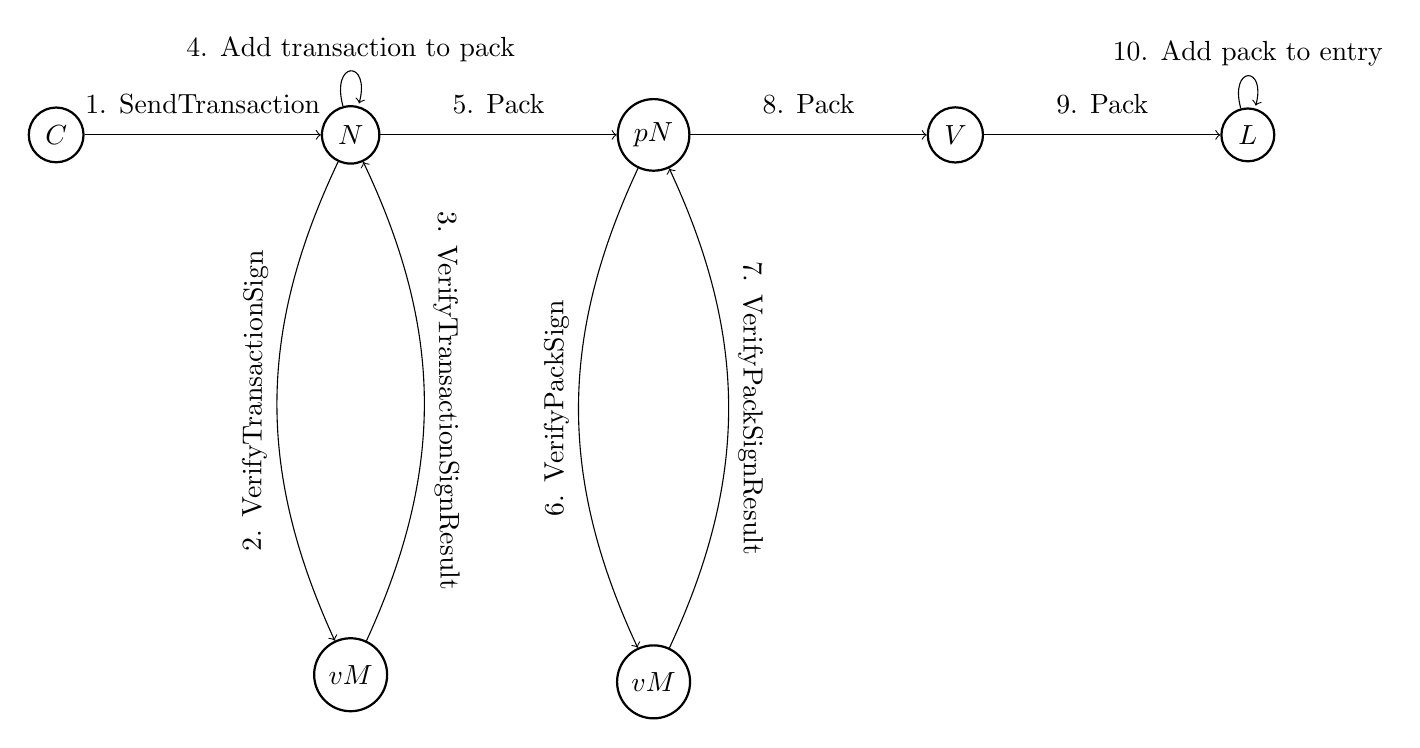
\begin{tikzpicture}[node distance={30mm}, main/.style = {circle, thick, draw}]
    \node[main] (1) {$C$}; 
    
    \node[main] (2) [right=30mm of 1] {$N$}; 
    \node[main] (3) [below=60mm of 2] {$vM$}; 
    
    \path[->] (1) edge node[above =0.15 cm] {1. SendTransaction} (2);
    \path[->] (2) edge[bend right = 25] node[midway, above, sloped] {2. VerifyTransactionSign} (3);
    \path[->] (3) edge[bend right = 25] node[midway, above, sloped] {3. VerifyTransactionSignResult} (2);
    
    \path (2) edge [loop above] node[above] {4. Add transaction to pack} (2);
    
    \node[main][right=30mm of 2](4) {$pN$}; 
    \path[->] (2) edge node[above=0.15 cm] {5. Pack} (4);

    \node[main] (5) [below=60mm of 4]{$vM$}; 
    \path[->] (4) edge[bend right = 25] node[midway, above, sloped] {6. VerifyPackSign} (5);
    \path[->] (5) edge[bend right = 25] node[midway, above, sloped] {7. VerifyPackSignResult} (4);

    \node[main] [right=30mm of 4](6) {$V$}; 
    \path[->] (4) edge node[above =0.15 cm] {8. Pack} (6);

    \node[main] [right=30mm of 6](7) {$L$}; 
    \path[->] (6) edge node[above =0.15 cm] {9. Pack} (7);
    \path (7) edge [loop above] node[above] {10. Add pack to entry} (7);

\end{tikzpicture} 

\section{Confirm flow}
\subsection{Create Vote flow}

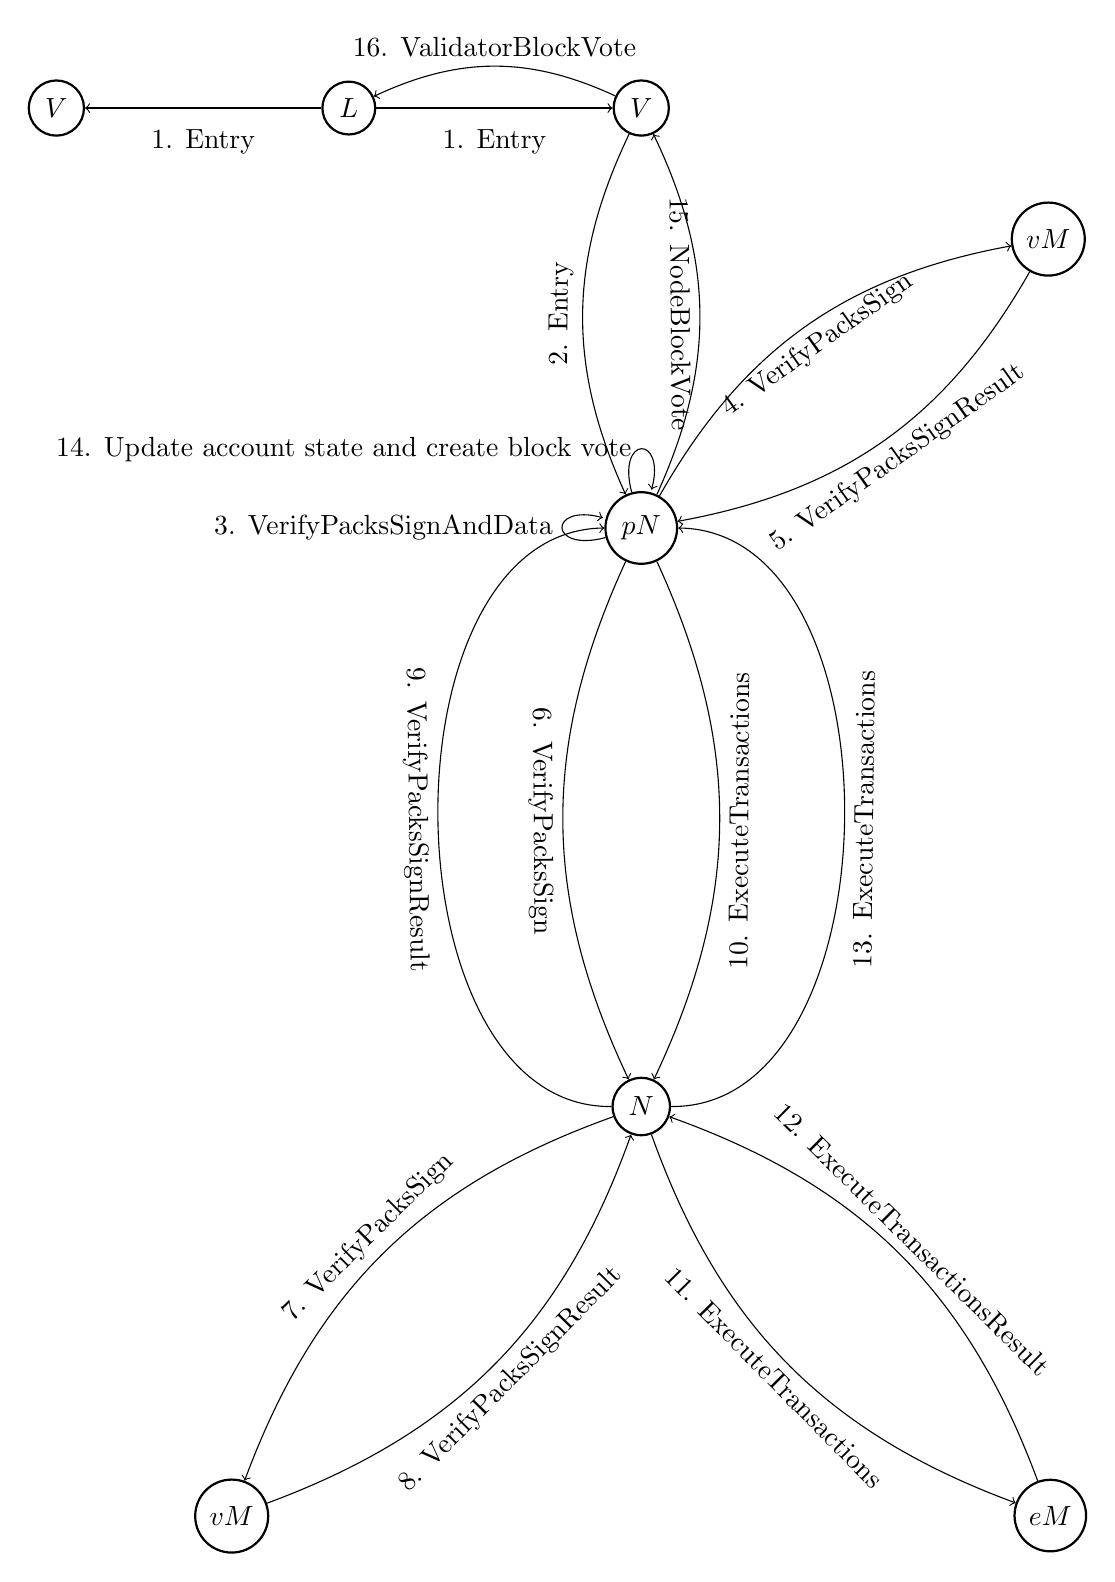
\begin{tikzpicture}[node distance={30mm}, main/.style = {circle, thick, draw}]
    \node[main] (1) {$L$}; 
    \node[main] (2) [left=30mm of 1] {$V$}; 
    \node[main] (3) [right=30mm of 1] {$V$}; 

    \path[->] (1) edge node[below =0.15 cm] {1. Entry} (2);
    \path[->] (1) edge node[below =0.15 cm] {1. Entry} (3);

    \node[main] (4) [below=45mm of 3] {$pN$}; 
    \path[->] (3) edge[bend right = 25] node[midway, above, sloped] {2. Entry} (4);
    \path (4) edge [loop left] node[left] {3. VerifyPacksSignAndData} (4);

    \node[main] (5) [ above right=30mm and 45mm of 4] {$vM$}; 
    \path[->] (4) edge[bend left = 25] node[midway, below, sloped] {4. VerifyPacksSign} (5);
    \path[->] (5) edge[bend left = 25] node[midway, below, sloped] {5. VerifyPacksSignResult} (4);


    \node[main] (6) [below=65mm of 4] {$N$}; 
    \path[->] (4) edge[bend right = 25] node[midway, below, sloped] {6. VerifyPacksSign} (6);

    \node[main] (7) [below left=65mm of 6] {$vM$}; 
    \path[->] (6) edge[bend right = 25] node[midway, above, sloped] {7. VerifyPacksSign} (7);
    \path[->] (7) edge[bend right = 25] node[midway, below, sloped] {8. VerifyPacksSignResult} (6);


    \path[->] (6) edge[bend left = 90] node[midway, below, sloped] {9. VerifyPacksSignResult } (4);
    \path[->] (4) edge[bend left = 25] node[midway, below, sloped] {10. ExecuteTransactions} (6);


    \node[main] (7) [below right=65mm of 6] {$eM$}; 

    \path[->] (6) edge[bend right = 25] node[midway, below, sloped] {11. ExecuteTransactions} (7);
    \path[->] (7) edge[bend right = 25] node[midway, above, sloped] {12. ExecuteTransactionsResult} (6);
    \path[->] (6) edge[bend right = 90] node[midway, below, sloped] {13. ExecuteTransactions} (4);

    \path (4) edge [loop above] node[left] {14. Update account state and create block vote} (4);

    \path[->] (4) edge[bend right = 25] node[midway, below, sloped] {15. NodeBlockVote} (3);
    \path[->] (3) edge[bend right = 25] node[midway, above, sloped] {16. ValidatorBlockVote} (1);
\end{tikzpicture} 
\pagebreak
\subsection{Consensus confirm block flow}
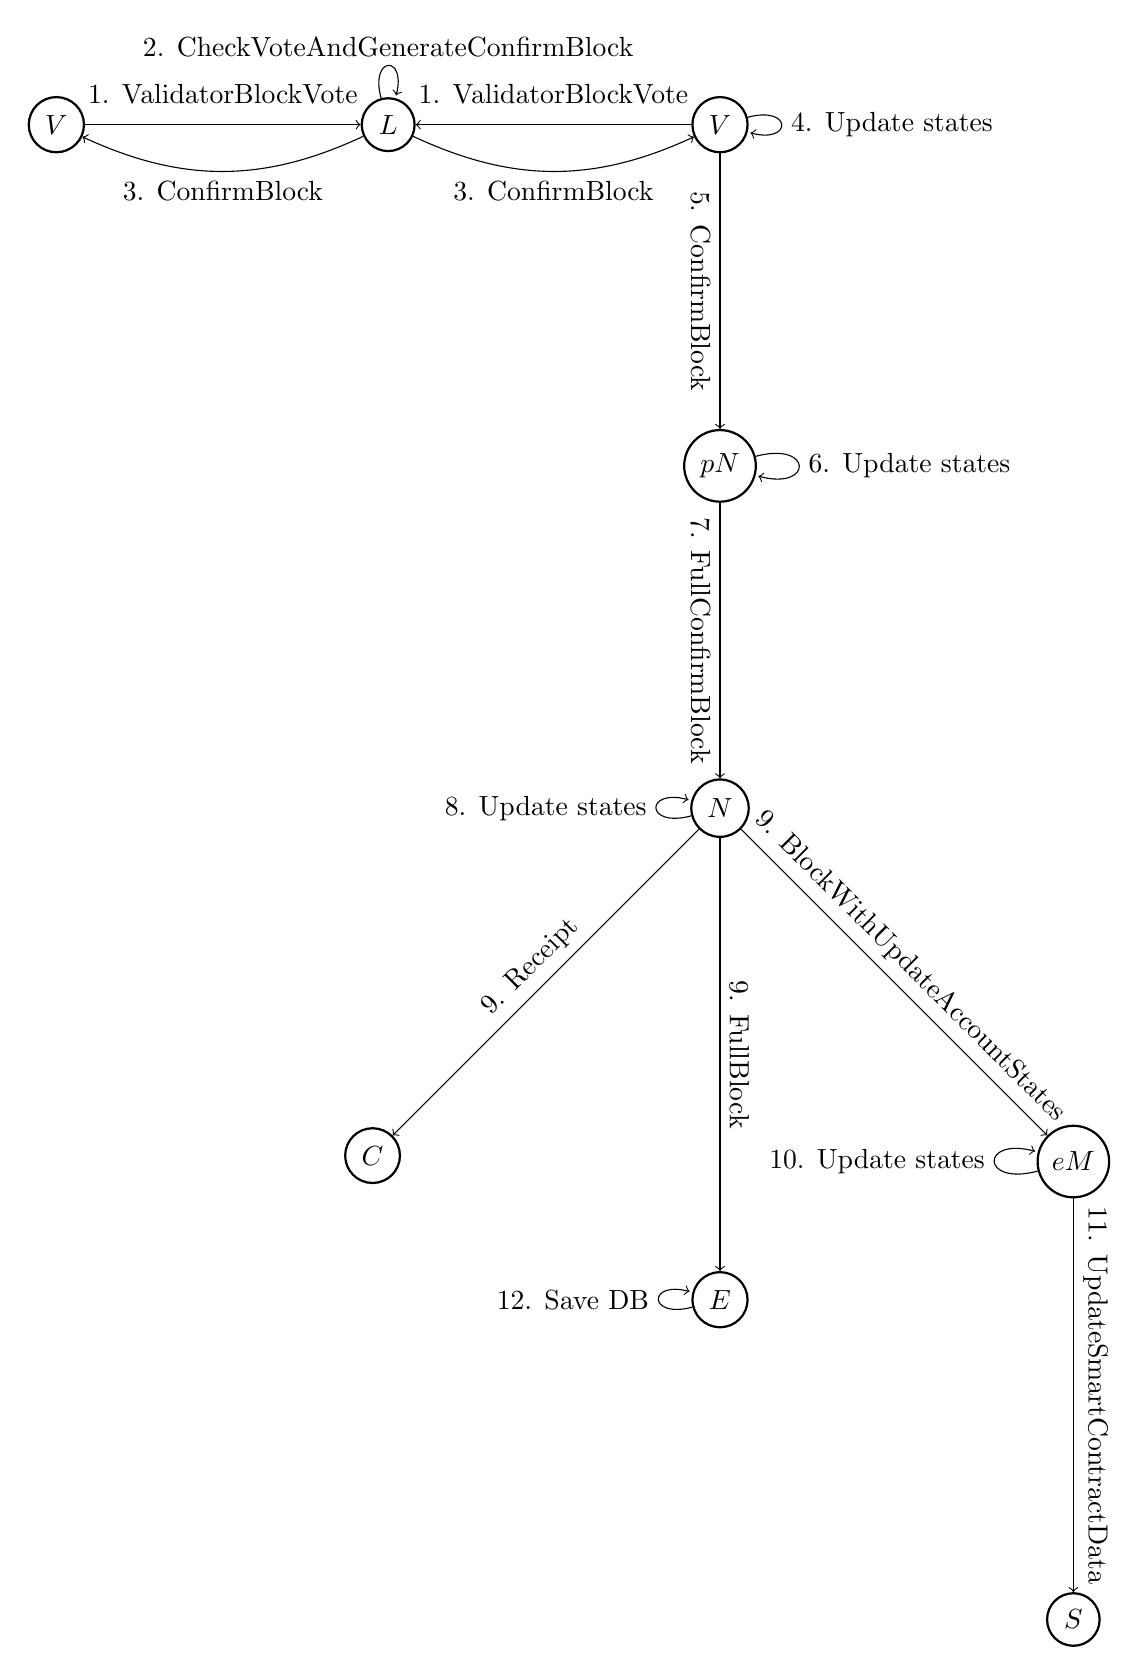
\begin{tikzpicture}[node distance={30mm}, main/.style = {circle, thick, draw}]
    \node[main] (1) {$L$}; 
    \node[main] (2) [left=35mm of 1] {$V$}; 
    \node[main] (3) [right=35mm of 1] {$V$}; 

    \path[->] (2) edge node[above =0.15 cm] {1. ValidatorBlockVote} (1);
    \path[->] (3) edge node[above =0.15 cm] {1. ValidatorBlockVote} (1);
    \path (1) edge [loop above] node[above] {2. CheckVoteAndGenerateConfirmBlock} (1);

    \path[->] (1) edge[bend left = 25] node[midway, below, sloped] {3. ConfirmBlock} (2);
    \path[->] (1) edge[bend right = 25] node[midway, below, sloped] {3. ConfirmBlock} (3);

    \path (3) edge [loop right] node[right] {4. Update states} (3);

    \node[main] (4) [below=35mm of 3] {$pN$}; 
    \path[->] (3) edge node[midway, below, sloped] {5. ConfirmBlock} (4);
    \path (4) edge [loop right] node[right] {6. Update states} (4);

    \node[main] (5) [below=35mm of 4] {$N$}; 
    \path[->] (4) edge node[midway, below, sloped] {7. FullConfirmBlock} (5);

    \node[main] (6) [below left=55mm of 5] {$C$}; 
    \node[main] (7) [below right =55mm of 5] {$eM$}; 
    \node[main] (8) [below =55mm of 5] {$E$}; 
    \path (5) edge [loop left] node[left] {8. Update states} (4);
    
    \path[->] (5) edge node[midway, above, sloped] {9. Receipt} (6);
    \path[->] (5) edge node[midway, above, sloped] {9. BlockWithUpdateAccountStates} (7);
    \path[->] (5) edge node[midway, above, sloped] {9. FullBlock} (8);

    \path (7) edge [loop left] node[left] {10. Update states} (7);

    \node[main] (9) [below =50mm of 7] {$S$}; 
    \path[->] (7) edge node[midway, above, sloped] {11. UpdateSmartContractData} (9);

    \path (8) edge [loop left] node[left] {12. Save DB} (8);


\end{tikzpicture} 
\bibliographystyle{abbrv}
% \bibliography{references}  % need to put bibtex references in references.xbib 
\end{document}
